% =============================================================================
%  Formal Runtime Verification for Tool-Using LLM Agents.
%  Offline same-benchmark replay on AgentDojo (recorded runs), STAC (recorded
%  chains) and R-Judge, with the real MonPoly engine.
%  Target venue: CPSIoTSec 2026 (co-located with ACM CCS). WiP short paper.
%  Build: tectonic main.tex  (fetches acmart).
% =============================================================================
\documentclass[sigconf]{acmart}

%% ---------------------------------------------------------------------------
%% ACM rights block. THE THREE VALUES BELOW MUST COME FROM THE ACM eRights
%% CONFIRMATION EMAIL FOR SUBMISSION #53 -- do not ship the placeholders.
%%   \setcopyright{...}  one of acmlicensed / acmcopyright / rightsretained /
%%                       usgov / cc  (the email states which)
%%   \acmDOI{...}        the assigned DOI
%%   \acmISBN{...}       the proceedings ISBN
%% Until the email arrives, `none' keeps the build clean and prints no false
%% rights statement.
\setcopyright{none}          %% TODO camera-ready: value from eRights email
%\acmDOI{10.1145/nnnnnnn.nnnnnnn}   %% TODO camera-ready: uncomment + real DOI
%\acmISBN{978-x-xxxx-xxxx-x/YY/MM}  %% TODO camera-ready: uncomment + real ISBN
\acmConference[CPSIoTSec '26]{Joint Workshop on CPS \& IoT Security and
  Privacy}{November 15, 2026}{The Hague, Netherlands}
\acmBooktitle{Joint Workshop on CPS \& IoT Security and Privacy (CPSIoTSec '26),
  November 15, 2026, The Hague, Netherlands}
\acmYear{2026}
%% printacmref=true is the ACM DL default for proceedings; confirmed pending with
%% the chairs (email_to_chairs.md, question 4). It costs ~10-14 lines at the foot
%% of column 1 on page 1.
\settopmatter{printacmref=true, printccs=true, printfolios=true}

\usepackage{booktabs}
\usepackage{microtype}
\usepackage{amsmath}
\let\Bbbk\relax
\usepackage{amssymb}
\usepackage{balance}
\usepackage{tikz}
\usetikzlibrary{arrows.meta,positioning}
\emergencystretch=3em

% Tighten the vertical space around floats (reduces the gap after Tables 1-3, etc.)
\setlength{\textfloatsep}{6pt plus 2pt minus 2pt}
\setlength{\floatsep}{6pt plus 2pt minus 2pt}
\setlength{\intextsep}{6pt plus 2pt minus 2pt}
\setlength{\dbltextfloatsep}{6pt plus 2pt minus 2pt}
\setlength{\dblfloatsep}{6pt plus 2pt minus 2pt}

\title[Formal Runtime Verification for Tool-Using LLM Agents]{Formal Runtime
       Verification for Tool-Using LLM Agents: An Offline Same-Benchmark Study
       on AgentDojo and STAC}

% Author list. Camera-ready 2026-08-26: the [anonymous] and [review] class
% options were removed, so this block now prints. Order: Kekatos first (per
% author agreement), all others alphabetical by surname. NB this differs from
% the order registered on HotCRP #53 -- update HotCRP to match before upload.
\author{Nikolaos Kekatos}
\affiliation{%
  \institution{Clone Systems}
  \city{Larnaca}\country{Cyprus}}

\author{Stylianos Basagiannis}
\affiliation{%
  \institution{International Hellenic University}
  \city{Serres}\country{Greece}}

\author{Marinelio Chintri}
\affiliation{%
  \institution{International Hellenic University}
  \city{Serres}\country{Greece}}

\author{Panagiotis Katsaros}
\affiliation{%
  \institution{Aristotle University of Thessaloniki}
  \city{Thessaloniki}\country{Greece}}

\author{Alexios Lekidis}
\affiliation{%
  \institution{University of Thessaly}
  \city{Larissa}\country{Greece}}

\author{Tom Nianios}
\affiliation{%
  \institution{Clone Systems}
  \city{Larnaca}\country{Cyprus}}

\author{Ioannis Seitoglou}
\affiliation{%
  \institution{International Hellenic University}
  \city{Serres}\country{Greece}}

\author{Anastasios Temperekidis}
\affiliation{%
  \institution{Clone Systems}
  \city{Larnaca}\country{Cyprus}}

\keywords{runtime verification, LLM agents, CPS/IoT security, tool-call
          monitoring, MonPoly, past-time temporal logic, agent guardrails}

\begin{CCSXML}
<ccs2012>
<concept>
<concept_id>10002978.10003022</concept_id>
<concept_desc>Security and privacy~Software and application security</concept_desc>
<concept_significance>500</concept_significance>
</concept>
<concept>
<concept_id>10003752.10003790</concept_id>
<concept_desc>Theory of computation~Logic and verification</concept_desc>
<concept_significance>300</concept_significance>
</concept>
<concept>
<concept_id>10010147.10010178.10010219</concept_id>
<concept_desc>Computing methodologies~Intelligent agents</concept_desc>
<concept_significance>300</concept_significance>
</concept>
</ccs2012>
\end{CCSXML}
\ccsdesc[500]{Security and privacy~Software and application security}
\ccsdesc[300]{Theory of computation~Logic and verification}
\ccsdesc[300]{Computing methodologies~Intelligent agents}

\begin{document}

\begin{abstract}
Guardrails for tool-using LLM agents are typically implemented as application-specific
rules, which makes multi-step, data-dependent policies hard to specify, audit and reuse.
We investigate metric first-order temporal logic (MFOTL) and its monitor
\textbf{MonPoly} as a declarative substrate for such policies, replaying the recorded
trajectories that AgentDojo, STAC and R-Judge already ship.

Five generic obligations flag $71.8\%$ of STAC chains and $70.1\%$ of GPT-4o's
\emph{successful} AgentDojo attacks, but also fire on $29.3\%$ of benign runs. Because
these corpora rarely record approvals and never record timestamps, the generic
obligations reduce to typed-action detection --- a benchmark-readiness gap for
history-dependent enforcement, which we quantify across the three corpora and answer with
a twelve-field enforcement-ready trace schema.

The value of MFOTL becomes clear with \emph{data-parametric} policies: payee-provenance
and external-recipient obligations substantially reduce benign firing while preserving
most detection. We then show that the provenance signal is itself attackable --- one
planted structured line defeats the check on $94$--$99\%$ of the runs it would otherwise
flag, deceiving no model, only the monitor --- and that binding provenance to the lookup
that produced it removes the evasion entirely at no cost in detection or benign firing. A
field ablation locates where each capability is gained, and shows that the sound and
unsound provenance policies are indistinguishable on clean traces, separating only under
attack. Finally, metric policies flip verdict on identical actions purely by elapsed time.

These results position MFOTL/MonPoly as an auditable substrate for relational and
temporal agent policies, complementary to rule-based enforcement, and locate the binding
constraint in the corpora rather than the formalism.
\end{abstract}

\maketitle

% ============================================================================
\section{Introduction}
\label{sec:intro}

The defences shipped with tool-using large language model (LLM) agents are, in
practice, mostly \emph{rule-based}. AgentSpec~\cite{agentspec2026}, Progent~\cite{progent2025} and
GuardAgent~\cite{guardagent2024} evaluate predicates on tool calls; the defences
benchmarked in AgentDojo~\cite{agentdojo2024} (tool filters, prompt spotlighting,
prompt repetition) are per-call or per-prompt heuristics. Some of these engines
maintain state, and with enough bespoke code a stateful rule can encode a
finite-history check --- so we do \emph{not} claim rules are incapable of
history-dependent enforcement. What they typically lack is a \emph{common
declarative semantics} for the multi-step, data-dependent policies that the
safety-relevant attacks exploit: each policy is re-encoded per application, in
imperative code, hard to audit, reuse, or verify. And those attacks are multi-step:
STAC reports attack-success above $90\%$ precisely because the violation is assembled
across a chain of individually-benign calls~\cite{stac2026}.

Monitoring a \emph{trace} against a declarative temporal specification is the
defining task of runtime verification. First-order temporal
monitors --- MonPoly~\cite{monpoly2014}, DejaVu~\cite{havelund2018dejavu} --- decide
metric, quantified past-time properties over event streams with data, which is the
exact shape of an agent obligation (``$\forall$ object $o$: an irreversible action
on $o$ requires a prior approval for $o$''). This makes metric first-order temporal
logic (MFOTL) and its monitor MonPoly a natural \emph{declarative substrate} for
such policies: quantified over data, with a formal
semantics and a reusable, independently-maintained engine, rather than bespoke
per-application code --- complementary to rule-based enforcement, not a claim that
rules cannot do it.

\paragraph{The empirical question} A paradigm argument is only as good as its
evidence: does formal RV actually catch \emph{real} agent attacks, and what does it
cost? Answering usually needs a live agent and an LLM. We avoid that: three major
benchmarks ship \emph{recorded} trajectories --- AgentDojo publishes $36.7$k
recorded runs (tool-call traces plus its own attack-success and utility labels),
STAC publishes $483$ recorded attack chains, and R-Judge~\cite{rjudge2024} ships
labelled agent records with an IoT subset. We can therefore run a real RV engine
over the \emph{same} benchmarks the community uses, entirely offline.

\paragraph{Central finding} The value of formal RV for agent traces depends as much on
what the trace \emph{records} as on what the specification language can \emph{express}.
On the corpora the community ships, generic temporal obligations collapse into
risky-action typing, because approvals, timestamps and state transitions are largely
absent; a keyword rule set would reach the same verdicts. Where relational or timing
context \emph{is} available, MFOTL buys genuinely more discriminating policies --- and
those policies then depend on trace content an attacker can write into. Provenance
integrity and benchmark instrumentation are therefore not side conditions but
prerequisites for history-dependent agent enforcement. That is the argument this paper
makes, and each contribution below is a step in it.

\paragraph{Contributions}
\begin{itemize}
\item \textbf{A declarative RV formulation for agent traces.} Five reusable agent
      obligations in MFOTL, with an offline same-benchmark pipeline that replays the
      trajectories AgentDojo, STAC and R-Judge already ship through the
      \emph{unmodified} MonPoly binary, scored against each benchmark's own labels
      (\S\ref{sec:oblig}, \S\ref{sec:method}).
\item \textbf{An empirical characterisation of when formal RV adds value.} Generic
      obligations achieve substantial attack coverage at a substantial benign firing
      cost, and largely reduce to typed-action detection because current corpora rarely
      record the history they quantify over. Data-parametric obligations, by contrast,
      improve discrimination by binding the verdict to prior payee or recipient
      provenance (banking benign firing $44\%\!\to\!24\%$, exact McNemar $p<10^{-10}$
      pooled across model directories), and metric policies flip verdict on identical
      actions purely by elapsed time (\S\ref{sec:results}--\S\ref{sec:cps}).
\item \textbf{The assurance conditions: what must be observable and trustworthy.}
      Provenance-based policies introduce a new attack surface --- one planted
      structured line reverses $94$--$99\%$ of affected verdicts, deceiving no model ---
      which we close by binding provenance to the lookup that produced it, at no cost in
      detection or benign firing. A field ablation shows sound and unsound provenance
      policies are indistinguishable on clean traces. And a readiness audit identifies
      the trace fields whose absence prevents current benchmarks from evaluating
      history-dependent enforcement at all, motivating a twelve-field enforcement-ready
      schema (\S\ref{sec:canon}--\S\ref{sec:gap}).
\end{itemize}

\paragraph{Scope} We measure whether an obligation \emph{fires on a recorded
trajectory} (detection under post-hoc replay), not live-agent attack success under an
in-loop shield. Studying an in-loop shield addresses a \emph{different} question ---
agent adaptation after enforcement --- outside the observational scope of this work.

% ============================================================================
\section{Background: Agent Guardrails and RV}
\label{sec:bg}

\paragraph{Rule-based agent guardrails} A per-call guardrail evaluates a
propositional predicate on the pending tool call. AgentSpec~\cite{agentspec2026}
and Progent~\cite{progent2025} give rule languages over the current call;
GuardAgent~\cite{guardagent2024} emits guard code from a knowledge base;
AgentDojo's built-in defences~\cite{agentdojo2024} filter tools or rewrite prompts;
Llama Guard~\cite{llamaguard2023} classifies message content. These are effective on
their target threats but reason over the current call (or prompt), not the
\emph{quantified past} of the trace, and each policy is re-encoded per application.

\paragraph{Benchmarks with recorded traces} AgentDojo~\cite{agentdojo2024}
evaluates prompt-injection attacks and defences across four suites (banking, slack,
travel, workspace) and \emph{ships} the resulting runs: per (model, suite, user
task, attack, injection) a JSON with the assistant tool-call trace and the labels
\textsf{security} (the injected task was accomplished) and \textsf{utility} (the
user task was accomplished). STAC~\cite{stac2026} ships $483$ recorded multi-turn
attack chains (derived from SHADE-Arena~\cite{shadearena2025} and
Agent-SafetyBench~\cite{agentsafetybench2024}), each a sequence of benign calls plus
a withheld final harmful step. R-Judge~\cite{rjudge2024} ships labelled agent
records across domains, including a smart-home / traffic / phone IoT subset. All are
replayable offline.

\paragraph{First-order temporal RV} MonPoly~\cite{monpoly2014} monitors MFOTL over
timed event streams, quantifying over data;
DejaVu~\cite{havelund2018dejavu} is a first-order past-time monitor and VeriMon is
MonPoly's formally verified core --- all drop-in for the past-time obligations here.
Stream monitors (RTLola~\cite{rtlola2019}, TeSSLa~\cite{tessla2018}) target numeric
signals and complement us for quantitative obligations. A \emph{hybrid} deployment
can route relational/parametric obligations to MonPoly and purely numeric ones to
RTLola/TeSSLa, reusing hybrid-hierarchical RV infrastructure that already runs both
families in edge-IoT settings~\cite{hybridhier2025,hiermon2026,critisfabric2026};
companion work of ours applies multi-aspect and compositional RV to LLM-enabled agents
and swarms in simulation~\cite{mesasagents2026,mesasswarm2026}, where the traces are
generated rather than recorded --- the complementary setting to the offline replay
studied here; a
shield~\cite{shielding2018} gates the pending call on a violation.

% ============================================================================
\section{Five Generic Obligations in MFOTL}
\label{sec:oblig}

We define five reusable obligations, each of the form ``a risky action of a given
class requires a matching precondition (approval/consent/confirmation) earlier in
the trace,'' chosen by action \emph{semantics} rather than any benchmark's tool
names: \textbf{O1}~irreversible/destructive (delete, cancel, purge),
\textbf{O2}~protection teardown (disable, unlock, add auto-delete rule),
\textbf{O3}~financial commit (transfer, pay, schedule transaction),
\textbf{O4}~external export (send, share, upload), and \textbf{O5}~actuation/config
(set, execute, adjust a device). In MFOTL (O1 shown; $\blacklozenge$ is
once-in-the-past):
\[
  \square\,\forall a.\ \big(\mathsf{destructive}(a)
    \rightarrow \blacklozenge\,\mathsf{approved}(a)\big).
\]
These are the specifications we hand to MonPoly (as their monitored violation form;
full formulas and keyword patterns in Appendix~\ref{app:repro}). They are
deliberately generic; the study measures how far five reusable formal templates go
on real benchmarks, and where precision then demands \emph{parametric} refinement
(binding the approval to the specific object, within a window) --- expressible in
MFOTL but not in stateless per-call predicates.

% ============================================================================
\section{Offline Same-Benchmark Methodology}
\label{sec:method}

\begin{figure}[t]
\centering
\resizebox{\columnwidth}{!}{%
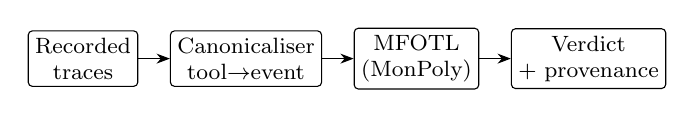
\begin{tikzpicture}[node distance=4mm, >=Stealth,
  b/.style={draw, rounded corners=1.5pt, align=center, inner sep=2.5pt,
            font=\footnotesize, minimum height=7mm}]
\node[b] (r) {Recorded\\traces};
\node[b, right=of r] (c) {Canonicaliser\\tool$\to$event};
\node[b, right=of c] (m) {MFOTL\\(MonPoly)};
\node[b, right=of m] (v) {Verdict\\+ provenance};
\draw[->] (r)--(c); \draw[->] (c)--(m); \draw[->] (m)--(v);
\end{tikzpicture}}
\caption{Offline pipeline. Recorded AgentDojo/STAC/R-Judge traces are canonicalised
to a typed event stream and checked against MFOTL obligations by MonPoly; verdicts
with provenance drive the offline analyses (coverage, BFR, earliest-warning,
provenance integrity). No LLM or agent is executed.}
\label{fig:pipeline}
\end{figure}

Figure~\ref{fig:pipeline} shows the offline pipeline.
\paragraph{Canonicalisation} For each recorded run we build one event stream from
the assistant tool calls (AgentDojo: \texttt{\{function,args\}} per call; STAC: the
interaction history plus the withheld final step; R-Judge: the agent-turn actions).
The monitor types each tool into an obligation class by semantic keyword patterns
and detects preconditions by approval patterns (Appendix~\ref{app:repro}).

\paragraph{Real engine} For STAC we additionally export the canonical stream to a
MonPoly log and the obligations to MFOTL, and run the \emph{unmodified MonPoly}
binary; its firings are the RV result, not a re-implementation. The CPS/IoT policies
of \S\ref{sec:cps} are likewise evaluated by MonPoly.

\paragraph{Why MonPoly} The obligations we need are not stateless predicates: they
quantify over trace data (payee identity, recipient domain) \emph{and} bound how far
back an enabler counts (consent within $24$\,h, three actuations in $6$\,h). That pair
of requirements --- first-order quantification plus \emph{metric past} --- is exactly
safe-range MFOTL, and MonPoly is a maintained implementation of it that runs
\emph{unmodified} on an exported log, so our headline firings are not a
re-implementation of our own semantics. Among the alternatives surveyed by the runtime
verification tools list,\footnote{\url{https://runtime-verification.github.io/tools.html}}
DejaVu~\cite{havelund2018dejavu} decides first-order past-time properties with BDDs but
offers no metric windows without its timed extension, so the bounded obligations would
not transfer directly; TeSSLa~\cite{tessla2018} and RTLola are stream-based and strong
on per-trace numeric computation, but weaker on the first-order joins over unbounded
domains (arbitrary payee and recipient strings) that the parametric obligations
require. VeriMon, a formally verified sibling of MonPoly, is a drop-in for the same
fragment and would be the natural choice where a machine-checked monitor is needed. We
therefore treat the engine as interchangeable within the fragment and the
\emph{specification} as the contribution.

\paragraph{Measures} On AgentDojo we use its labels: over attacked runs,
\emph{detection on successful attacks} (of \textsf{security}$=$true runs, the
fraction where an obligation fires) and the \emph{benign firing rate} (BFR: of benign
runs, the fraction where an obligation fires). BFR is a potential-block proxy for the
utility cost --- what a shield \emph{would} gate --- not a measured task-failure rate,
which would require re-running the agent. On STAC (attack-only) we
report \emph{final-step detection} (fires on the withheld harmful step); on R-Judge,
detection on unsafe records and false-positive rate on safe ones. Confidence
intervals are Wilson $95\%$ score intervals.

\paragraph{Benign sampling and parameter choice} The unit is one recorded run. A
benign run is one user task with \emph{no} injection ($\approx\!30$ per suite, so
$123$ benign GPT-4o runs with a parseable trace); an attacked run is a (user
task~$\times$~injection~$\times$~attack) combination ($6680$). The benign set is thus
small, and we report Wilson intervals on every rate (e.g.\ the $29.3\%$ aggregate BFR
has interval $[24.1,40.4]$). The keyword patterns are the ordinary English verbs for
each class (Appendix~\ref{app:repro}), fixed \emph{before} measuring outcomes and
never adjusted; the one threshold, the $\blacklozenge$ window, is the most permissive
choice (unbounded past), so a firing is never a tight-window artefact. ``Detection''
means the obligation fires on the recorded call; a would-be shield gating it assumes
prevention. STAC's content-semantic failure modes (harmful free text) are out of
structural scope and flagged, if at all, only via the delivery act.

\emph{One correction to the frozen set.} The approval list originally contained the
token \texttt{ack}, intended for acknowledgement tools. Because matching is on
substrings it also matched \texttt{invite\_user\_to\_slack} and
\texttt{remove\_user\_from\_slack} --- $595$ calls in the Slack suite --- each of which
then acted as a prior approval and suppressed every later obligation in that run. The
pattern \texttt{authorize} likewise matched the read-only lookup
\texttt{list\_authorized\_personnel}. We corrected both after the fact: \texttt{ack} is
now spelled \texttt{acknowledge}, and no read-only accessor (prefix \texttt{get\_},
\texttt{list\_}, \texttt{read\_}, \texttt{search\_}, \texttt{view\_}, \texttt{fetch\_} or
\texttt{query\_}) can constitute an approval event. The correction \emph{raises} the
reported rates --- AgentDojo detection $61.6\%\!\to\!70.2\%$, Slack-suite detection
$40.3\%\!\to\!63.9\%$, BFR $31.7\%\!\to\!32.5\%$ --- so the pre-correction figures
understated the method rather than inflating it, and every number reported here is from
the corrected set. STAC and R-Judge are unaffected: no tool name in either corpus
collides. We report the correction rather than silently re-freezing, because it is
precisely the class of error a substring canonicaliser invites and precisely what
\S\ref{sec:canon} sets out to measure.

% ============================================================================
\section{Results}
\label{sec:results}

\paragraph{AgentDojo (same-benchmark, offline)} Table~\ref{tab:agentdojo} replays
all recorded GPT-4o runs (no defence). AgentDojo's own no-defence attack-success is
$28.9\%$ ($1931/6680$). Our RV, applied to the identical runs, fires on $70.1\%$
($95\%$ CI $[68.1,72.2]$) of the \emph{successful} attacks --- i.e.\ a shield would
have had a flagged call to gate in nearly two-thirds of the attacks that actually got
through --- driven mostly by the financial, export and actuation obligations
(teardown never fires: these suites have no teardown tools). The cost is real and we
report it plainly: the same generic obligations fire on $29.3\%$ ($36/123$, Wilson
$95\%$ $[22.0,37.8]$) of \emph{benign} task runs, because a legitimate task also sends
email, moves money and changes config. Detection and BFR rise and fall together under
\emph{generic} specs.

Two caveats belong here rather than in a later limitations block. First, \emph{what
these numbers do and do not demonstrate}: because AgentDojo and STAC record almost no
approval events and no timestamps (\S\ref{sec:gap}, Table~\ref{tab:score}), the
approval antecedent of O1--O5 is vacuously unsatisfied --- after the correction noted in
\S\ref{sec:method}, no AgentDojo tool call matches it at all --- and a firing therefore
depends only on the tool's class. At this layer MFOTL is buying declarative uniformity, not
temporal reasoning: a typed-action keyword rule set would reach the same verdicts. The
claims that do rest on the formalism are the parametric obligations of
\S\ref{sec:param}, the timed policies of \S\ref{sec:cps}, and the benchmark scorecard
of \S\ref{sec:gap}. Second, \emph{a $29.3\%$ BFR is not a deployable operating point}.
BFR counts runs on which some obligation fires; it is a firing proxy, not a measured
utility cost, since we never re-execute the blocked task to see whether it would still
have succeeded. At this rate the generic layer is a triage filter for human review, not
an enforcement gate, and the benign sample ($123$ runs) is small enough that the
interval above is wide.

\begin{table}[t]
\centering
\caption{AgentDojo recorded runs (GPT-4o, no defence), replayed offline through our
MFOTL obligations. Detection is on AgentDojo's \textsf{security}=true (successful)
attacks; BFR is on its benign (\textsf{attack}=none) runs. The per-obligation counts
\emph{overlap} --- one run can trip several obligations --- so they sum to $1677$, more
than the $1354$ runs detected; the union, not the sum, is the detection figure. Runs
whose tool-call chain is empty or unparseable are excluded ($96$ of $6899$, all in
banking). Fuller breakdown in Appendix~\ref{app:extended},
Table~\ref{tab:peroblig}.}
\label{tab:agentdojo}
\renewcommand{\arraystretch}{1.1}
\setlength{\tabcolsep}{5pt}
\begin{tabular}{lc}
\toprule
Measure & value \\
\midrule
Attacked runs                                  & $6680$ \\
AgentDojo attack-success (no defence)          & $1931/6680 = 28.9\%$ \\
RV detection on \emph{successful} attacks       & $1354/1931 = 70.1\%$ \\
RV fires on any attacked run                     & $2292/6680 = 34.3\%$ \\
RV BFR on benign runs                     & $36/123 = 29.3\%$ \\
\quad Wilson $95\%$ interval on BFR             & $[22.0,37.8]$ \\
\midrule
\multicolumn{2}{l}{\emph{by obligation, on the $1354$ detected (overlapping)}} \\
\quad destructive without confirmation         & $307$ \\
\quad teardown without approval                & $0$ \\
\quad financial without confirmation           & $518$ \\
\quad export without consent                   & $539$ \\
\quad actuation without precondition           & $313$ \\
\quad sum of the five (overlap $>$ union)       & $1677$ \\
\bottomrule
\end{tabular}
\end{table}

\paragraph{Across models} The pattern is not GPT-4o-specific: across the
$22$ base (no-defence) model directories AgentDojo ships, RV detection on successful
attacks spans $40.9$--$83.3\%$ and BFR $17.6$--$37.4\%$. AgentDojo's own built-in
defences are not comparable to our offline replay, since they execute the agent
\emph{with} the defence in the loop, whereas we never re-run the agent.

\paragraph{Earliest warning: when the obligation fires (prevention timing)} A
detection is only useful for prevention if it arrives before the harmful step. On the
$1931$ successful GPT-4o AgentDojo attacks, an obligation fires \emph{before} the
final harmful call (\emph{preventive}) in $1012$ ($52.4\%$), fires only \emph{at} that
call (\emph{last-moment}) in $342$ ($17.7\%$), and never fires in $577$ ($29.9\%$);
where it is preventive the median detection lead is one tool-call (mean $2.19$, max
$13$). On STAC the picture inverts by construction --- the corpus \emph{withholds} the
final harmful step, so the signal concentrates there: $76/483$ ($15.7\%$) preventive,
$278$ ($57.6\%$) last-moment, $129$ ($26.7\%$) no firing. The earliest-warning margin,
not a post-hoc residual, is our intervention-timing evidence.

\paragraph{Per suite: where generic obligations break down} The suite breakdown
(Appendix~\ref{app:extended}, Table~\ref{tab:suite}) exposes the precision problem
concretely. In \textbf{banking}, every action is a financial commit, so the generic
obligations flag $97.4\%$ of successful attacks \emph{and} $79.2\%$ of benign runs --- near-total
recall at near-total BFR. Travel, with few money/export actions, is the opposite
($16.5\%$ detection, $11.1\%$ BFR). No single generic threshold is right for all
suites; the domain-specific \emph{parametric} refinements (\S\ref{sec:param}) are what
recover precision.

\paragraph{STAC (recorded chains, MonPoly)} Table~\ref{tab:stac} replays all
$483$ STAC chains. Our reference monitor flags the withheld harmful action in
$347/483 = 71.8\%$ ($95\%$ CI $[67.7,75.7]$) of chains, and the \emph{unmodified
MonPoly engine}, fed the MFOTL obligations and the exported log, fires on
\emph{exactly} the same $347$ --- the engine confirms the result. On the
structurally-intended failure modes the rate is $72.8\%$; the content-semantic modes
(harmful text, trusting/filtering tool results, $\approx$$29\%$ of cases) are out of
structural scope and flagged only via the delivery act. $136$ chains end in an action
outside the five generic classes (spam-rule edits, calendar changes, in-place
appends), mapping where new obligations or semantics are needed.

\begin{table}[t]
\centering
\caption{STAC recorded chains ($483$) replayed through the same obligations;
final-step detection. The MonPoly engine reproduces the $347$ firings exactly.}
\label{tab:stac}
\renewcommand{\arraystretch}{1.1}
\setlength{\tabcolsep}{5pt}
\small
\begin{tabular}{lc}
\toprule
Measure & value \\
\midrule
Final-step detection (ref.\ monitor)        & $347/483 = 71.8\%$ \\
\quad confirmed by \textbf{MonPoly}          & $347$ (exact) \\
\quad structural-intent modes                 & $249/342 = 72.8\%$ \\
Out-of-template misses                         & $136$ \\
Content-semantic (needs semantics)            & $141\ (\approx\!29\%)$ \\
\bottomrule
\end{tabular}
\end{table}

\paragraph{R-Judge: the structural limit on a broad safety benchmark} To probe where
structural RV runs out, we replay the \emph{full} R-Judge~\cite{rjudge2024} --- $571$
records ($301$ unsafe, $270$ safe), a genuine benign set unlike STAC. The generic
obligations fire on $23.6\%$ ($71/301$) of unsafe records at $16.3\%$ ($44/270$) FPR.
The low detection is expected: most R-Judge unsafe cases are \emph{content-semantic}
(privacy leakage, misinformation, unsafe advice) with no structural trace signature,
so a rule-based per-call checker fares no better. R-Judge thus \emph{bounds} the reach
of structural trace-level RV --- formal or rule-based alike --- and confirms a semantic
aspect is the necessary complement.

% ============================================================================
\section{Parametric Obligations: the Centrepiece}
\label{sec:param}

The AgentDojo BFR is not an artefact of RV --- it afflicts \emph{any}
action-type checker, rule-based or formal, because ``sends email'' is both the attack
and the job. Closing it needs a \emph{precise} condition that quantifies over trace
data: allow the transfer only if a matching approval for \emph{that} payee occurred,
or the export only if the recipient came from the user's own directory. Such
conditions are expressible in MFOTL and monitorable by MonPoly, and are \emph{not
expressible as a stateless per-call predicate}, which cannot refer to the payee's
past provenance. We are careful here: a \emph{stateful} rule engine could of course
compute the same condition procedurally, by accumulating seen payees in bespoke code.
The advantage we claim is therefore not exclusive computability but \emph{declarative
specification} --- one formula, with formal temporal/relational semantics, evaluated
by a reusable, independently-maintained engine, and hence auditable --- rather than
per-application imperative state management. We implement two and measure them
(Table~\ref{tab:param}).

\paragraph{Payee provenance (banking)} Instead of firing on \emph{any} transfer
(generic O3), the parametric obligation fires only on a transfer to a payee never
seen as a \emph{structured} recipient/sender in prior account data,
\[
  \square\,\forall p.\ \big(\mathsf{transfer}(p)\wedge
    \neg\,\blacklozenge\,\mathsf{known\_payee}(p)\big).
\]
On GPT-4o banking runs this cuts the benign firing rate from $44.0\%$ to $24.0\%$ while
detection on successful attacks falls only from $79.2\%$ to $70.0\%$: the injected
attacker IBAN is embedded in free text and is never a real counterparty, so it is
still flagged, whereas a legitimate transfer to a known payee no longer is.

\paragraph{External recipient (workspace)} Symmetrically for export, the parametric
obligation fires only on a \texttt{send\_email} whose recipient never appeared as a
structured directory entry (contact/participant/sender field) in a prior tool result,
\[
  \square\,\forall r.\ \big(\mathsf{send}(r)\wedge
    \neg\,\blacklozenge\,\mathsf{known\_contact}(r)\big).
\]
The injection payload delivers the attacker address inside a free-text email body,
not the directory, so it is treated as external; a colleague already in the calendar
or address book is not. This cuts the workspace BFR from $15.2\%$ to $10.9\%$ at a
detection cost of $42.5\%\!\to\!39.2\%$.

\paragraph{Discrimination} The positive likelihood ratio $\mathrm{LR^+}$
(detection $/$ BFR) summarises both error rates in one number. Refining the generic
obligations ($\mathrm{LR^+}=2.40$) to the parametric spec raises it on both suites ---
payee provenance $1.80\!\to\!2.92$, external recipient $2.79\!\to\!3.61$ --- so the
parametric conjunct separates benign from malicious transfers/exports better than
typed-action detection.

\paragraph{Statistical significance} The parametric obligation is a strict refinement
of the generic one, so the paired comparison is concordant except for the discordant
cell where the generic fires but the parametric does not. Single-model denominators
are too small to be conclusive; pooling benign runs across all AgentDojo model
directories ($700$ banking, $1{,}376$ workspace) makes every discordant run a
reduction (banking $75$ vs $0$, workspace $37$ vs $0$), with detection largely
preserved. The exact McNemar test is then $p=5.3\times10^{-23}$ (banking) and
$p=1.5\times10^{-11}$ (workspace).

\begin{table}[t]
\centering
\caption{Parametric vs.\ generic obligations (GPT-4o), with Wilson $95\%$ intervals.
Every row is a \emph{single} obligation on a \emph{single} suite --- not a policy-set
union, so these rates are not comparable with the pooled run-level figures of
Appendix~\ref{app:extended}. The parametric rows fire only when a
relational/provenance condition over the trace holds, so their verdict differs from
the same call's typed-action verdict; the generic detection numbers elsewhere are
typed-action detection. Benign denominators: $25$ banking runs ($11/25$ and $6/25$)
and $46$ workspace runs ($7/46$ and $5/46$), counting every run with a non-empty
message list. On the identical $46$ workspace runs the generic \emph{union} of
Table~\ref{tab:suite} fires on $10/46=21.7\%$, against $7/46=15.2\%$ for O4 alone ---
the clearest illustration that the two tables report different policy sets, not
different data.}
\label{tab:param}
\renewcommand{\arraystretch}{1.15}
\setlength{\tabcolsep}{4pt}
\footnotesize
\begin{tabular}{llcc}
\toprule
Suite & Spec & detect \% [CI] & BFR \% [CI] \\
\midrule
banking   & generic O3          & $79.2\ [75.7,82.3]$ & $44.0\ [26.7,62.9]$ \\
banking   & param.\ payee       & $70.0\ [66.1,73.6]$ & $24.0\ [11.5,43.4]$ \\
workspace & generic O4          & $42.5\ [38.3,46.8]$ & $15.2\ [7.6,28.2]$  \\
workspace & param.\ ext-recip.\ & $39.2\ [35.1,43.5]$ & $10.9\ [4.7,23.0]$  \\
\bottomrule
\end{tabular}
\end{table}

\paragraph{What depends on temporal/parametric reasoning} We are explicit about the
provenance of each number. The generic O1--O5 detection and BFR rates
(Tables~\ref{tab:agentdojo}--\ref{tab:stac}) are \emph{typed-action detection}: a
firing depends only on the tool's class, not on trace history, because approvals are
almost never present in these corpora. The two parametric rows in
Table~\ref{tab:param}, and every verdict flip in the CPS/IoT study
(\S\ref{sec:cps}), \emph{do} depend on genuine relational or temporal reasoning: the
\emph{same} call is allowed or flagged according to a prior-provenance or
prior-state condition --- which a \emph{stateless} per-call predicate cannot decide,
and which MFOTL states declaratively rather than leaving to bespoke stateful code.

% ============================================================================
\section{Canonicalisation: Accuracy and Sensitivity}
\label{sec:canon}

Detection is only as good as the tool$\to$class typing. A single annotator, blind to
the typing predictions and to any detection outcome, hand-labelled $54$ distinct tool
names sampled stratified by call frequency and domain across AgentDojo and STAC.
Against this gold set the keyword typing has micro-averaged precision and recall both
$0.87$ and single-primary exact-match $87.0\%$ ($47/54$); the residual errors are
systematic (e.g.\ \texttt{send\_\allowbreak channel\_\allowbreak message} missed by
export, read-only \texttt{get\_*\_transactions} false-typed financial) rather than
random, and we report rather than tune them (per-class table in
Appendix~\ref{app:extended}, Table~\ref{tab:canon}). To bound how much this typing
drives the headline numbers, we re-ran the replays under four tool$\to$class mappings
(original, corrected, conservative, expanded; Table~\ref{tab:canonsens}): AgentDojo
detection moves in $[69.0,79.9]\%$ and BFR in $[26.0,43.9]\%$, STAC detection stays in
$[61.7,73.1]\%$ --- moderately sensitive, with the frozen typing \emph{conservative}
on AgentDojo (correcting the mapping raises detection, not lowers it).

% ============================================================================
\section{Provenance Integrity: the Monitor's Trace History is an Attack Surface}
\label{sec:prov}

The parametric obligations of \S\ref{sec:param} draw their power from a
\emph{provenance} predicate --- \textsf{known\_payee}, \textsf{known\_contact} ---
computed over the monitor's own recorded trace: a payee is trusted iff it appeared
earlier as a structured recipient/sender field. That trace is, however, partly
attacker-controlled: an injection can plant text that the canonicaliser reads as a
structured directory entry, so the history the monitor trusts is itself an attack
surface.

\paragraph{Poisoning the provenance signal} We test this directly, injecting one line
naming the attacker recipient into each flagged run's readable context in four framings.
A \emph{structured} directory line or a \emph{quoted/forwarded} line flips $94.0\%$ of
the $403$ flagged banking-payee runs and $99.0\%$ of the $203$ flagged
workspace-recipient runs to ``known'' (no longer flagged); a \emph{free-text} mention
and a \emph{reformatted} recipient flip $0\%$ (per-framing counts in
Appendix~\ref{app:extended}). One planted structured or quoted line therefore defeats
the provenance check for $94$--$99\%$ of the transfers it would otherwise flag: the
check trusts \emph{syntactic} structure it cannot authenticate.

\paragraph{A hardened provenance specification} The fix is to make provenance
integrity part of the specification. A hardened obligation should require that
(i) provenance come from a \emph{trusted tool result} (an account/directory API
response), not message text; (ii) a trusted contact \emph{predate the session};
(iii) an approval \emph{bind to the exact payee and amount}, not the action class; and
(iv) a \emph{new} payee require explicit confirmation. Conditions (i)--(iv) are
themselves MFOTL obligations over a suitably-typed trace (a trust-domain field, a
session id, an approval bound to object and amount) --- exactly the schema current
benchmarks lack (\S\ref{sec:gap}).

Conditions (ii)--(iv) need fields the corpora do not carry, so they remain design
proposals. Condition (i) does not, once stated precisely, and we therefore
\emph{evaluate} it. Note first that the obvious reading of (i) is vacuous against this
attacker: the injection is itself a forged tool result, and the workspace obligation
already restricts accrual to tool messages, yet still flips $99\%$. What discriminates is
\emph{call--answer binding} --- a genuine tool result answers a lookup the agent itself
issued, whereas a planted message answers nothing outstanding:
\[
\mathit{known}(p)\;\leftrightarrow\;\ooalign{$\bullet$\cr}\bigl(\mathit{lookup}(t)\wedge
\raisebox{0pt}{$\bigcirc$}\,\mathit{result}(t,p)\bigr).
\]
Re-running the same four perturbations against this hardened predicate
(Table~\ref{tab:harden}) removes the evasion entirely --- structured and quoted framings
fall from $94.0\%$ to $0.0\%$ on banking and $99.0\%$ to $0.0\%$ on workspace --- at
\emph{no} cost: detection ($403/576$ banking, $203/518$ workspace) and benign firing
($6/25$, $5/46$) are unchanged to the run. The fix is not a precision/robustness
trade-off; the naive predicate was simply reading a field it had no warrant to trust. We
claim this for the tested attack family only: an attacker who can forge a matching
lookup call, or compromise the tool being queried, is outside its reach.

\begin{table}[t]
\centering
\caption{Hardened provenance against the poisoning attack of \S\ref{sec:prov}: flip rate
(flagged runs whose verdict reverses to ``known''). Detection and benign firing are
identical under both predicates, so the hardening costs nothing measurable here.}
\label{tab:harden}
\renewcommand{\arraystretch}{1.05}
\setlength{\tabcolsep}{5pt}
\footnotesize
\begin{tabular}{llcc}
\toprule
Suite & planted line & naive & hardened \\
\midrule
banking ($403$ flagged)   & structured        & $94.0\%$ & $\mathbf{0.0\%}$ \\
                          & quoted/forwarded  & $94.0\%$ & $\mathbf{0.0\%}$ \\
                          & free text         & $0.0\%$  & $0.0\%$ \\
                          & reformatted       & $0.0\%$  & $0.0\%$ \\
\midrule
workspace ($203$ flagged) & structured        & $99.0\%$ & $\mathbf{0.0\%}$ \\
                          & quoted/forwarded  & $99.0\%$ & $\mathbf{0.0\%}$ \\
                          & free text         & $0.0\%$  & $0.0\%$ \\
                          & reformatted       & $0.0\%$  & $0.0\%$ \\
\bottomrule
\end{tabular}
\end{table} Provenance integrity is a first-class requirement for agent
RV, not a canonicalisation detail.

% ============================================================================
\section{CPS/IoT Case Study: Timed Temporal Policies}
\label{sec:cps}

This is a proof of \emph{applicability} of MFOTL/MonPoly to CPS/IoT policies,
not a broad security validation on CPS/IoT deployments. We give three evidence points,
all evaluated verbatim by MonPoly: \emph{timed} (metric) actuation policies, a
multi-instance building trace, and a real (small) IoT subset.

\paragraph{Timed policies whose verdict depends on elapsed time} A reviewer of an
earlier version noted the generic obligations exercise little temporal complexity ---
on these corpora an unbounded $\blacklozenge$ reduces to typed-action detection. We
therefore author three \emph{metric} obligations whose verdict on the \emph{identical}
action changes purely with the clock (signatures, logs and formulas in
Appendix~\ref{app:repro}; Table~\ref{tab:timed}). \emph{(T1) Bounded-window consent}:
an export requires a consent within the last $W{=}24$\,h,
$\mathsf{export}(o)\wedge\neg(\text{\textsc{once}}[0,24]\,\mathsf{consent}(o))$ ---
MonPoly fires only when the consent is stale. \emph{(T2) Sliding-window rate limit}:
$\ge 3$ actuations on a device within $W{=}6$\,h (metric \textsc{cnt} over
$\text{\textsc{once}}[0,6]$) --- fires on a burst, silent once calls are spaced.
\emph{(T3) Timed precedence}: an \texttt{execute} must be preceded within $W{=}8$\,h by
an authorisation --- fires only when the authorisation has expired. Each is exactly
the kind of ``property that contains time'' a per-call classifier, and an unbounded
past-time check, cannot express.

\begin{table}[t]
\centering
\caption{Timed (metric MFOTL) policies evaluated verbatim by MonPoly. For each, the
\emph{same} action is allowed or a violation purely by elapsed time; $\bullet$ marks
the timepoints where MonPoly fires. Full sig/log/formula in Appendix~\ref{app:repro}.}
\label{tab:timed}
\renewcommand{\arraystretch}{1.1}
\setlength{\tabcolsep}{5pt}
\footnotesize
\begin{tabular}{llc}
\toprule
Policy (window) & action, timing & MonPoly \\
\midrule
T1 consent ($24$\,h)   & export, consent $12$\,h ago      & pass \\
T1 consent ($24$\,h)   & export, consent $48$\,h ago      & $\bullet$ \textbf{violation} \\
T1 consent ($24$\,h)   & export, re-consent $10$\,h ago   & pass \\
T2 rate ($\ge3/6$\,h)  & 3rd actuation within $6$\,h      & $\bullet$ \textbf{violation} \\
T2 rate ($\ge3/6$\,h)  & actuations spaced $>6$\,h apart  & pass \\
T3 precede ($8$\,h)    & execute, auth $6$\,h ago         & pass \\
T3 precede ($8$\,h)    & execute, auth $40$\,h ago        & $\bullet$ \textbf{violation} \\
T3 precede ($8$\,h)    & execute, re-auth $4$\,h ago      & pass \\
\bottomrule
\end{tabular}
\end{table}

The traces behind Table~\ref{tab:timed} are likewise authored, not recorded: the point
they establish is that \emph{elapsed time alone} flips MonPoly's verdict on an
otherwise identical action, which is a property of the specification language, not
evidence of field accuracy.

\paragraph{Multi-instance building actuation} To show the effect is not a single
hand-picked pair, we author a $20$-event smart-building trace ($13$ policy-relevant
actions) exercising three past-time policies with multiple compliant and violating
instances each (envelope-plus-maintenance-mode, a timed actuator dependency, and
badge-authorised access; formulas in Appendix~\ref{app:repro}). MonPoly flags exactly
the $6$ history-violating instances and clears all $7$ compliant ones; one violation
is a purely \emph{timed} miss --- an enabling \texttt{damper\_open} that fell $4$\,h
before a $3$\,h window --- so the same compressor start is a violation only by timing.

\paragraph{R-Judge IoT (real data, small --- cannot be enlarged)} The R-Judge IoT
subset (smart home, traffic dispatch, phone) is \emph{all the labelled IoT agent
records the benchmark ships}: $30$ records ($19$ unsafe, $11$ safe), so we report it as
illustrative. The generic obligations yield $31.6\%$ detection ($6/19$) and $27.3\%$
FPR ($3/11$) with wide Wilson intervals. It does contain relational cases: in one
unsafe record the agent grants a dog-walker \emph{permanent} smart-lock access without
consent. Encoding it under a parametric consent obligation
$\square\,\forall g,p.(\mathsf{grant}(g,p)\wedge p{=}1\wedge
\neg\,\blacklozenge\,\mathsf{consent}())$, MonPoly fires on the permanent grant and
clears once a prior consent is present --- a verdict flip on real IoT data the generic
``grant'' typing (which never fires here) cannot make.

% ============================================================================
\section{Benchmark Readiness for History-Dependent Agent Enforcement}
\label{sec:gap}

Our experiments expose a broader evaluation problem. Current agent-security benchmarks
record enough to determine whether an \emph{attack succeeded}, but not enough to
evaluate many \emph{history-dependent enforcement} policies. We therefore assess the
three corpora as enforcement datasets, and quantify the availability of the state,
provenance, approval and timing information a runtime monitor quantifies over. This is
not a criticism of their design --- they were built to measure attack success and agent
behaviour, which they do well --- but a statement that they are not, as shipped,
\emph{enforcement-ready}. The consequence is the phenomenon we reported in
\S\ref{sec:results}: with the history absent, sophisticated temporal obligations
necessarily collapse into simple action typing. A readiness scorecard over the three
benchmarks (Table~\ref{tab:score}) makes this concrete. Explicit \emph{approvals} are almost absent --- $0/6899$ ($0\%$)
AgentDojo events, $6/483$ ($1.2\%$) STAC chains, $1/571$ ($0.2\%$) R-Judge records.
Recipient/payee identity is recoverable more often ($38.8\%$/$58.4\%$/$5.8\%$) and
object identity sometimes ($36.4\%$/$34.2\%$/$47.3\%$), but user-confirmation events
are rare ($4.6\%$/$16.4\%$/$0\%$). Above all, \emph{none} of the three carries real
timestamps (only call order), structured state transitions, or reversibility typing.
The metric and stateful policies that motivate temporal RV (\S\ref{sec:cps}) thus
cannot be evaluated on these corpora as shipped --- we authored timed logs to exercise
them. As a practical consequence we derive a twelve-field \emph{enforcement-ready} trace
schema --- the twelve fields tabulated in Table~\ref{tab:score} --- being the minimum
event semantics needed to
benchmark relational, provenance-sensitive and timed policies. Recording these fields is
cheap at trace-emission time --- every one is available to the harness at the moment a
tool is called --- and it is what would let the next generation of corpora evaluate this
class of defence at all. One caveat follows from the census below: fields are necessary
but not sufficient. A single-turn benchmark cannot express approval however many columns
its log has, so an enforcement-ready corpus is a claim about the \emph{interaction
protocol} as much as about the schema.

\paragraph{Why the approvals are absent} The natural objection is that we search for
approvals by \emph{tool name} and may simply be looking in the wrong place. We therefore
looked everywhere, and the attrition is itself the result. Two structural facts explain
it. AgentDojo is \emph{single-turn}: exactly one user message per run
($6899/6899$), stating a task up front, after which the agent executes autonomously. An
approval is by definition a response to a \emph{proposed} action, which requires a user
turn \emph{after} the proposal; the protocol has no such turn, and consistently none of
its $68$ distinct tools is approval-like. Approvals there are foreclosed by the
interaction protocol, not merely unrecorded --- no parser can recover them. STAC is
\emph{multi-turn} (mean $2.6$ user turns, up to five), so approvals \emph{can} occur, and
approval language does appear: mining the user text rather than tool names raises the
count twelvefold, from $6/483$ ($1.2\%$) to $70/483$ ($14.5\%$) on a loose keyword match
and $39/483$ ($8.1\%$) on a strict permission-granting match. But only $3/483$ ($0.6\%$)
occur \emph{before} the harmful step, which is the only position from which an approval
could gate anything --- because STAC's attacks work precisely by smuggling the harmful
step in without returning to the user. Better extraction therefore does not rescue the
situation: it relocates the shortfall from recording to \emph{protocol and position}. An
enforcement-ready corpus needs an interaction shape in which approval is expressible, not
just a field in which it could be written down.

\paragraph{What each field buys} A scorecard says which fields are missing; it does not
say what capability their absence costs. We therefore ablate the trace itself, masking
fields cumulatively on AgentDojo banking and asking, at each level, which policy class
remains evaluable and how well it discriminates (Table~\ref{tab:ablation}). Two results
stand out. First, the levels the corpora \emph{do} support are exactly the ones that buy
little: recipient identity lifts $\mathrm{LR^+}$ from $1.80$ to $2.92$, and then the
approval- and timing-dependent levels are simply unevaluable --- \emph{zero}
approval-typed calls and \emph{zero} timestamped messages across $1545$ runs. Second, and
less obviously, R1 and R2 are \emph{observationally identical} on clean traces: same
detection, same benign firing, same $\mathrm{LR^+}$. They separate only under attack, at
$94\%$ versus $0\%$ evasion. Field availability alone therefore does not tell you whether
a provenance policy is sound; the binding does, and its value is invisible to any
evaluation that does not include an adversary. This is the sharper form of the readiness
argument: a corpus can expose every field a policy names and still be unable to
distinguish a sound policy from an unsound one.

\begin{table}[t]
\centering
\caption{Trace-field ablation on AgentDojo banking. Levels are cumulative; ``poison
flip'' is the structured-line evasion rate of \S\ref{sec:prov}. R1 and R2 differ only
under attack.}
\label{tab:ablation}
\renewcommand{\arraystretch}{1.05}
\setlength{\tabcolsep}{4pt}
\footnotesize
\begin{tabular}{llccc}
\toprule
Level & policy class & detect & BFR & flip \\
\midrule
R0 action only        & typed-action O1--O5   & $79.2\%$ & $44.0\%$ & --- \\
R1 $+$ recipient id   & recipient-bound       & $70.0\%$ & $24.0\%$ & $94\%$ \\
R2 $+$ bound provenance & poison-resistant    & $70.0\%$ & $24.0\%$ & $\mathbf{0\%}$ \\
\midrule
R3 $+$ approval binding & approval-bound      & \multicolumn{3}{c}{unevaluable: $0$ approvals$/1545$ runs} \\
R4 $+$ timestamps/state & metric, transition  & \multicolumn{3}{c}{unevaluable: $0$ timestamped messages} \\
\bottomrule
\end{tabular}
\end{table}

\begin{table}[t]
\centering
\caption{Benchmark readiness for history-dependent enforcement: fraction of
runs/records exposing each field. Real timestamps, structured state transitions, and
reversibility typing are absent from all three (call-order only).}
\label{tab:score}
\renewcommand{\arraystretch}{1.1}
\setlength{\tabcolsep}{5pt}
\small
\begin{tabular}{lccc}
\toprule
Field & AgentDojo & STAC & R-Judge \\
\midrule
explicit approval      & $0\%$    & $1.2\%$  & $0.2\%$  \\
recipient/payee id     & $38.8\%$ & $58.4\%$ & $5.8\%$  \\
object id              & $36.4\%$ & $34.2\%$ & $47.3\%$ \\
user confirmation      & $4.6\%$  & $16.4\%$ & $0\%$    \\
real timestamps        & none     & none     & none     \\
structured state       & none     & none     & none     \\
reversibility typing   & none     & none     & none     \\
\bottomrule
\end{tabular}
\end{table}

\paragraph{A minimal trace schema} We therefore propose a minimal enforcement-ready
schema --- twelve fields per event: \texttt{timestamp}, \texttt{actor}, \texttt{tool},
\texttt{action}, \texttt{object}, \texttt{recipient}, \texttt{source},
\texttt{approval\_id}, \texttt{session\_id}, \texttt{state\_before},
\texttt{state\_after}, \texttt{trust\_domain}. Current benchmarks supply the middle
group (tool/action, partially object/recipient) but none of wall-clock
\texttt{timestamp}, \texttt{approval\_id}, \texttt{session\_id}, the state pair, or
\texttt{trust\_domain} --- the fields the timed policies (\S\ref{sec:cps}) and the
hardened provenance spec (\S\ref{sec:prov}) require. Cheap to emit but absent
everywhere, they are the concrete obstacle to evaluating history-dependent agent
enforcement.

% ============================================================================
\section{Discussion and Conclusion}
\label{sec:concl}

\paragraph{Positioning} Table~\ref{tab:matrix} (appendix) contrasts the paradigms
\emph{as demonstrated in the cited work and its evaluated configurations}, not as a
fundamental-impossibility claim. AgentDojo~\cite{agentdojo2024},
AgentBench~\cite{agentbench2024} and ToolEmu~\cite{toolemu2023} \emph{evaluate} agents;
the guardrails they benchmark are, as reported, per-call or rule-based.
AgentSpec~\cite{agentspec2026} has a formal rule semantics and some history-aware rules
($\circ$), so a determined encoding could reach further than the cells show. Formal RV
combines trace-level scope, formal temporal semantics, data-parametric provenance, and
offline evaluability in \emph{one} declarative substrate --- not that the others
provably cannot.

\paragraph{Limitations} We measure firing on recorded trajectories, not live-agent
prevention; an in-loop shield addresses a different question (agent adaptation after
enforcement) outside our scope, and one we pursue separately with a digital-twin-in-the-loop
harness~\cite{mesasdtloop2026}. Generic specs have a high BFR ($29.3\%$), and the
parametric refinements that reduce it are evaluated for banking and workspace only.
STAC lacks preconditions ($6/483$ chains), so its generic obligations reduce to
typed-action detection; the metric power of MFOTL is exercised in the CPS/IoT study
instead. Keyword typing is coarse, and a semantic residual ($\approx$$29\%$ of STAC,
more of R-Judge) needs a content checker structural RV does not provide. Finally, the
timed policies run the real MonPoly engine but on authored logs that isolate the
timing dependence --- establishing expressiveness, not field prevalence.

\paragraph{Conclusion} Offline on real agent-attack corpora, MonPoly flags $71.8\%$ of STAC chains and
detects $70.1\%$ of GPT-4o's successful AgentDojo attacks at $29.3\%$ BFR --- numbers
that mostly reflect risky-action \emph{typing}, since these corpora rarely contain the
preconditions temporal logic is for. Where data-parametric and timed reasoning applies,
MFOTL states and MonPoly checks conditions a stateless per-call predicate cannot. Three
completed results anchor the security case: a concrete earliest-warning margin
(preventive on $52.4\%$ of successful AgentDojo attacks, median lead one tool-call);
the provenance predicate behind the parametric precision is itself an attack surface,
flipped $94$--$99\%$ by one planted structured line, for which we sketch --- but, on
these corpora, cannot yet evaluate --- a hardened trusted-provenance specification; and
a readiness scorecard showing current benchmarks
lack the timestamps, structured state, reversibility typing and approvals
history-dependent enforcement needs. That last result is the one we would most want
carried forward: widely used agent-security corpora support attack-level evaluation but
systematically omit the event semantics required to test history-dependent enforcement.
It explains why generic temporal policies collapse to action typing on current corpora,
and it motivates the enforcement-ready trace schema of \S\ref{sec:gap} as the concrete
thing a future benchmark could adopt. MFOTL/MonPoly is thus a reusable, auditable
substrate for quantified, timed agent-trace policies, complementary to rule-based
enforcement and measurable offline on the corpora the community already ships.

\balance
\bibliographystyle{ACM-Reference-Format}
\bibliography{references}

% ============================================================================
\appendix
\raggedbottom
\section{Reproducibility}
\label{app:repro}
\sloppy
This appendix is excluded from the page limit. All scripts are pure-stdlib Python in
\texttt{agent-rv-impl/}; the datasets are the public releases below.

\paragraph{Datasets} STAC (arXiv:2509.25624,
\texttt{amazon-science/\allowbreak Mul\-ti\-Turn\-Agent\-Attack},
$483$ chains, file \texttt{STAC\_\allowbreak benchmark\_\allowbreak data.json}); AgentDojo
(\texttt{ethz-spylab/\allowbreak agentdojo}, recorded
\texttt{runs/\allowbreak<model>/\allowbreak<suite>/...}, $\approx$$36.7$k
runs; we use \texttt{gpt-4o-2024-05-13} in detail and, for the cross-model analysis,
the $22$ base (no-defence) model directories the release ships, plus their defence
variants where pooled --- $28$ directories with a banking suite and $29$ with a
workspace suite);
R-Judge (\texttt{Lordog/R-Judge}, \texttt{data/}, $571$ records; the IoT subset
\texttt{data/IoT/\{household,trafficdispatch,phone\_iot\}.json} is all $30$ IoT
records the benchmark ships and cannot be enlarged offline).

\paragraph{Keyword patterns (typing)} A tool matches a class iff its lower-cased name
contains any listed substring.
\emph{DESTRUCTIVE:} delete, remove, cancel, clear, wipe, drop, purge, erase, revoke,
uninstall.
\emph{TEARDOWN:} autodelete, disable, stop, unlock, deactivate, turn\_off, bypass,
whitelist, allowlist, add\_user\_autodelete.
\emph{FINANCIAL:} send\_money, transaction, transfer, payment, pay\_, book\_, buy,
purchase, zelle, venmo, wire, invoice, checkout.
\emph{EXPORT:} send\_email, share, export, upload, post\_, publish, forward,
sendmessage, send\_message, send\_sms, tweet.
\emph{ACTUATION:} set\_, adjust, trafficlight, unlock\_door, execute, terminal,
medication, open\_, close\_, activate, reboot, restart, deploy, write\_, update\_,
configure, install.
\emph{APPROVAL (precondition):} confirm, approve, consent, authorize, authorise,
permission, verify, grant, two\_factor, 2fa, otp, request\_approval, ack, sign\_off,
double\_check.

\paragraph{Argument normalisation} Tool arguments are parsed from JSON to a dict
(malformed strings kept under a raw key). The \texttt{known\_payee} and
\texttt{known\_contact} predicates are \emph{not} hand-curated: they are emitted by
the same scripted canonicaliser via a fixed regular expression over structured
recipient/sender fields, and the regexes were frozen \emph{before} we inspected any
attacker IBAN/address or any \textsf{security}/\textsf{utility} outcome. For the payee
obligation a recipient is a \emph{known payee} only if it matched
\texttt{(?:recipient|\allowbreak sender):\allowbreak\textbackslash s*\allowbreak([A-Z]\{2\}\allowbreak[0-9A-Z]\{6,\})}
in prior message text (a structured IBAN field, not free text). For the external-recipient
obligation an address is a \emph{known contact} only if it appeared under a directory
key \texttt{(?:from|\allowbreak sender|\allowbreak recipients?|\allowbreak participants?|\allowbreak email|\allowbreak shared\_with|\allowbreak owner):}
in a prior \emph{tool} result. So a payee/contact becomes ``known'' purely by the
scripted rule, independent of whether it is later an attack address.

\paragraph{Approval/consent recognition} An approval precedes step $i$ iff some call
at $j<i$ (same trace, same STAC case) matches the APPROVAL patterns. An obligation
fires on step $i$ iff the tool matches its class patterns \emph{and} no approval
precedes $i$.

\paragraph{Timestamps and multiple firings} Each canonical event becomes one MonPoly
timepoint \texttt{@t}; for STAC the class and \texttt{approval} predicates are
parameterised by the case id so \texttt{ONCE} only matches within a case. Only
timepoints that carry at least one typed predicate are emitted: a canonicalised step
whose tool matches \emph{no} obligation class (a read-only or out-of-template action)
produces no event, so the log holds $357$ predicate-bearing timepoints across the
$483$ cases, and cases whose final step matches no class emit nothing and cannot fire
(counted as a miss). Because the STAC obligations use an unbounded
$\text{\textsc{once}}[0,10^6]$, dropping predicate-free timepoints is sound --- an
unbounded past-time operator is insensitive to the number of intervening empty
timepoints, only to whether a matching predicate occurred earlier in the case. For the
\emph{timed} policies of \S\ref{sec:cps} this is different: there the integer
timestamp is the event's clock time (in hours), timepoints are spaced by real elapsed
time, and the metric windows ($\text{\textsc{once}}[0,W]$) depend on those gaps, so we
keep the actual times rather than a dense index. Per-obligation counts are
non-exclusive; a case/run counts as detected if $\ge 1$ obligation fires.

\paragraph{Full MFOTL obligations (monitored violation form)} With
$\blacklozenge$ once-in-the-past:
\begin{align*}
&\text{O1}: \mathsf{destructive}(a)\wedge\neg\,\blacklozenge\,\mathsf{approved}(a)\\
&\text{O2}: \mathsf{teardown}(a)\wedge\neg\,\blacklozenge\,\mathsf{approved}(a)\\
&\text{O3}: \mathsf{financial}(a)\wedge\neg\,\blacklozenge\,\mathsf{approved}(a)\\
&\text{O4}: \mathsf{export}(a)\wedge\neg\,\blacklozenge\,\mathsf{approved}(a)\\
&\text{O5}: \mathsf{actuation}(a)\wedge\neg\,\blacklozenge\,\mathsf{approved}(a)
\end{align*}
The STAC export uses the disjunction handed verbatim to MonPoly:
\texttt{(destructive(c) OR teardown(c) OR financial(c) OR export(c) OR
actuation(c)) AND NOT (ONCE[0,1000000] approval(c))}.
The two parametric obligations are $\square\forall p.(\mathsf{transfer}(p)\wedge
\neg\blacklozenge\mathsf{known\_payee}(p))$ and
$\square\forall r.(\mathsf{send}(r)\wedge\neg\blacklozenge\mathsf{known\_contact}(r))$.
The multi-instance building policies, run verbatim by MonPoly, are:
\begin{quote}\ttfamily\footnotesize\raggedright
P1: setpoint(z,v) AND v > 28 AND NOT ((NOT maint\_off()) SINCE maint\_on())\\
P2: compressor\_start(z) AND NOT (ONCE[0,3] damper\_open(z))\\
P3: door\_unlock(d) AND NOT (ONCE[0,3] badge\_auth(d))\\
lock: grant\_access(g,p) AND p = 1 AND NOT (ONCE consent())
\end{quote}
The $20$-event building log yields firings at timepoints
$\{4,5,9,14,19,22\}$ ($6$ violations; the P2 firing at $t{=}14$ is the timed miss,
a \texttt{damper\_open} at $t{=}10$ outside the $3$-unit window) and no firing on the
$7$ compliant instances.

\paragraph{Timed (metric) policies of \S\ref{sec:cps}} These use hour-valued
timestamps; formula, signature and log are run verbatim by MonPoly:
\begin{quote}\ttfamily\footnotesize\raggedright
T1: export(o) AND NOT (ONCE[0,24] consent(o))\\
\hspace*{1em}log: @0 consent(1) @12 export(1) @48 export(1) @50 consent(1) @60 export(1)\\
\hspace*{1em}$\Rightarrow$ fires only @48 (consent 48h stale)\\
T2: (c <- CNT s; d (ONCE[0,6] actuate(d,s))) AND c >= 3\\
\hspace*{1em}log: @0 actuate(7,1) @2 actuate(7,2) @5 actuate(7,3) @30.. @33.. @40..\\
\hspace*{1em}$\Rightarrow$ fires only @5 (3rd actuation within 6h; spaced calls never fire)\\
T3: execute(x) AND NOT (ONCE[0,8] request(x))\\
\hspace*{1em}log: @0 request(5) @6 execute(5) @40 execute(5) @44 request(5) @48 execute(5)\\
\hspace*{1em}$\Rightarrow$ fires only @40 (authorisation 40h old)
\end{quote}
Each timed verdict flips on the \emph{same} action purely by elapsed time; T2 uses
MonPoly's metric \texttt{CNT} aggregation over a sliding $[0,6]$ window.

\paragraph{MonPoly version and invocation} The engine is MonPoly, version string
\texttt{MonPoly (development build)} (from \texttt{monpoly -version}), at
\texttt{/usr/local/bin/monpoly} inside Docker image \texttt{rv-fabric-impl-backend}
(image id \texttt{sha256:6e223674\allowbreak66a8}). It is invoked as
\texttt{monpoly -sig <s>.sig -formula <f>.mfotl -log <l>.log}; all formulas above pass
\texttt{monpoly -check} as monitorable. On the STAC export it fires on exactly $347$
timepoints, matching the reference monitor. Because both consume the same canonical log,
that agreement checks our implementation rather than the specification, so we add a
genuinely independent engine. \textbf{DejaVu}~\cite{havelund2018dejavu} decides
first-order past-time properties by a different procedure (BDDs over quantified
past-time LTL). The STAC obligation is untimed past-time first order, so it transfers to
DejaVu's QTL without weakening; on the same event stream DejaVu reports exactly $347$
violations. We additionally run \textbf{VeriMon}~\cite{verimon2022}, MonPoly's formally
verified kernel (\texttt{monpoly -verified}), whose monitoring algorithm is
machine-checked in Isabelle/HOL: also exactly $347$. So the obligation is agreed by four
monitors --- our reference implementation, MonPoly's standard kernel, its verified
kernel, and an independently developed BDD-based engine --- of which the last two make
the result something stronger than agreement between MonPoly and a checker we wrote
ourselves: one is a different decision procedure, and one is proved correct.

\paragraph{Artifact availability} All evaluation scripts are pure-stdlib Python under
\texttt{agent-rv-impl/}; together with the MonPoly signature/log/formula files for the
STAC, building, IoT and timed studies they will be released as supplementary material
%% TODO camera-ready: the paper is no longer anonymous, so this must name a real,
%% resolvable repository. github.com/nikos-kekatos/formal-rv-tool-using-llm-agents
%% is still PRIVATE as of 2026-08-26 -- make it public and insert the URL, or drop
%% the clause. Do not ship "anonymous public repository" in a signed paper.
(and a public repository), so the full pipeline is
reproducible against the public dataset releases named above.

\paragraph{AgentDojo selection and unflagged successful-attack fraction} Runs are read
by recursive glob of \texttt{runs/<model>/**/*.json}. A run is \emph{attacked} iff
\texttt{attack\_type} is set and $\neq$\texttt{none} and \texttt{injection\_task\_id}
is present; \emph{benign} iff neither is present; runs with an empty/unparseable
tool-call chain are skipped ($96$ for GPT-4o $\Rightarrow 6680$ attacked, $123$
benign). \texttt{security==True} marks a successful attack, \texttt{utility==True} a
completed task. For reference we report the \emph{unflagged successful-attack
fraction}, $(\textsf{successful}\wedge\neg\textsf{RV-fired})/\textsf{attacked}
=(1931-1354)/6680=8.6\%$; this is a descriptive count of successful attacks the
monitor did not flag, \emph{not} a measured attack-success rate under an in-loop
shield (which would require re-running the agent).

% ============================================================================
\section{Extended Results and Robustness}
\label{app:extended}

\begin{table}[htbp]
\centering
\caption{Paradigm comparison, \emph{per each system's evaluated configuration} (not a
fundamental-capability claim). TL = trace-level; FS = formal temporal semantics;
PAR = parametric (quantifies over trace data); OFF = evaluable offline on recorded
runs. $\circ$ = partial / achievable with bespoke stateful code.}
\label{tab:matrix}
\renewcommand{\arraystretch}{1.1}
\setlength{\tabcolsep}{5pt}
\footnotesize
\begin{tabular}{lcccc}
\toprule
                                  & TL & FS & PAR & OFF \\
\midrule
AgentDojo defences~\cite{agentdojo2024} & --         & --         & --         & \checkmark \\
AgentSpec~\cite{agentspec2026}    & $\circ$    & \checkmark & $\circ$    & -- \\
Progent~\cite{progent2025}        & $\circ$    & --         & --         & -- \\
GuardAgent~\cite{guardagent2024}  & --         & --         & --         & -- \\
STAC~\cite{stac2026} (benchmark)  & \checkmark & --         & --         & \checkmark \\
\textbf{Formal RV / MonPoly (ours)} & \checkmark & \checkmark & \checkmark & \checkmark \\
\bottomrule
\end{tabular}
\end{table}

\paragraph{Per-obligation ablation (AgentDojo, GPT-4o)} Table~\ref{tab:peroblig}
breaks the union result down by obligation, with each obligation's positive likelihood
ratio $\mathrm{LR^+}$ (detection $/$ BFR). Export is the single most discriminating
obligation ($\mathrm{LR^+}=2.58$) and teardown never fires for GPT-4o (these suites
have no protection-teardown tools).

\begin{table}[htbp]
\centering
\caption{Per-obligation detection on successful attacks and BFR (AgentDojo, GPT-4o),
with unique flagged successful attacks and $\mathrm{LR^+}=$ detection/BFR. Union is the
headline any-obligation result.}
\label{tab:peroblig}
\renewcommand{\arraystretch}{1.0}
\setlength{\tabcolsep}{5pt}
\small
\begin{tabular}{lcccc}
\toprule
Obligation & detect \% & BFR \% & unique & $\mathrm{LR^+}$ \\
\midrule
O1 destructive & $15.9$ & $4.1$  & $259$ & $3.91$ \\
O2 teardown    & $0$    & $0$    & $0$   & --     \\
O3 financial   & $26.8$ & $13.0$ & $243$ & $2.06$ \\
O4 export      & $27.9$ & $10.6$ & $491$ & $2.64$ \\
O5 actuation   & $16.2$ & $6.5$  & $38$  & $2.49$ \\
\midrule
union (any)    & $70.1$ & $29.3$ & --    & $2.40$ \\
\bottomrule
\end{tabular}
\end{table}

\begin{table}[htbp]
\centering
\caption{Per-suite replay (GPT-4o, no defence): AgentDojo attack-success, RV detection
on successful attacks, and RV BFR on benign runs. Detection and BFR here are
\emph{policy-set unions} over all five generic obligations, so they exceed the
single-obligation rates of Table~\ref{tab:param} on the same suite: workspace BFR is
$10/46$ as a union against $7/46$ for O4 alone. This table also counts only runs with
a non-empty tool-call chain ($96$ banking runs are excluded on that ground, one of them
benign), whereas Table~\ref{tab:param} counts every run with a non-empty message list:
the banking gap therefore has two causes at once. Under the message-list filter the
generic union fires on $19/25=76.0\%$ of benign banking runs against $19/24=79.2\%$
here, the same numerator over the one extra run; Table~\ref{tab:param}'s $11/25$ differs
from both because it is a single obligation rather than the union.}
\label{tab:suite}
\renewcommand{\arraystretch}{1.0}
\setlength{\tabcolsep}{6pt}
\small
\begin{tabular}{lccc}
\toprule
Suite & ASR & RV detect & BFR \\
\midrule
banking   & $40.1\%$ & $97.4\%$ & $79.2\%$ \\
slack     & $60.9\%$ & $63.9\%$ & $15.4\%$ \\
travel    & $9.3\%$  & $16.5\%$ & $11.1\%$ \\
workspace & $19.9\%$ & $62.9\%$ & $21.7\%$ \\
\bottomrule
\end{tabular}
\end{table}

\paragraph{Cross-model sign test (parametric payee, banking)} Beyond the pooled
McNemar test (\S\ref{sec:param}), we check the direction of the parametric effect
per model. Across the $22$ base (no-defence) model directories with a banking suite,
the parametric payee obligation \emph{decreases} benign firing in $20$, leaves it
unchanged in $2$, and increases it in $0$; the median per-directory reduction is
$8.0$ percentage points (IQR $[4,17]$, min $0$, max $24$). An exact two-sided sign
test on the $20$-vs-$0$ split gives $p=1.9\times10^{-6}$: the reduction direction is
consistent across models, not an artefact of pooling. Over the same $22$ directories,
generic detection ranges $40.9$--$83.3\%$ and BFR $17.6$--$37.4\%$.

\begin{table}[htbp]
\centering
\caption{Canonicalisation typing vs.\ $54$ hand-labelled tools. Per-class multi-label
precision/recall (does the typing include the gold class?), micro-average, and
single-primary exact-match.}
\label{tab:canon}
\renewcommand{\arraystretch}{1.0}
\setlength{\tabcolsep}{6pt}
\small
\begin{tabular}{lccc}
\toprule
Class & P & R & (tp/fp/fn) \\
\midrule
O1 destructive & $0.78$ & $1.00$ & $7/2/0$ \\
O2 teardown    & $1.00$ & $1.00$ & $3/0/0$ \\
O3 financial   & $0.78$ & $0.78$ & $7/2/2$ \\
O4 export      & $1.00$ & $0.67$ & $4/0/2$ \\
O5 actuation   & $0.86$ & $0.86$ & $6/1/1$ \\
\midrule
micro-average  & $0.90$ & $0.84$ & F1 $0.87$ \\
\multicolumn{4}{l}{single-primary exact-match: $47/54 = 87.0\%$} \\
\bottomrule
\end{tabular}
\end{table}

\paragraph{Canonicalisation sensitivity} Table~\ref{tab:canonsens} re-runs the
AgentDojo and STAC replays under four tool$\to$class mappings. Correcting the known
typing errors raises detection and BFR together (the frozen keyword typing is
conservative); the conservative mapping leaves AgentDojo unchanged but lowers STAC.

\begin{table}[htbp]
\centering
\caption{Sensitivity of the headline rates to the tool$\to$class mapping. AD =
AgentDojo (GPT-4o); STAC detection is final-step.}
\label{tab:canonsens}
\renewcommand{\arraystretch}{1.0}
\setlength{\tabcolsep}{6pt}
\small
\begin{tabular}{lccc}
\toprule
Mapping & AD detect \% & AD BFR \% & STAC detect \% \\
\midrule
original      & $70.1$ & $29.3$ & $71.8$ \\
corrected     & $79.9$ & $43.9$ & $73.1$ \\
conservative  & $69.0$ & $26.0$ & $61.7$ \\
expanded      & $79.9$ & $43.9$ & $73.1$ \\
\bottomrule
\end{tabular}
\end{table}

\paragraph{MonPoly runtime and scale-up soundness} Table~\ref{tab:runtime} reports
throughput and peak resident memory for the STAC log at $1\times$, $10\times$ and
$50\times$ replication and for an AgentDojo-derived log. Throughput is dominated by
start-up on short logs, rising from $52$--$179$k events/s on the $357$-timepoint STAC
log to $0.36$--$0.46$M at $\times10$--$\times50$ and $0.8$M on the AgentDojo export,
with flat $8$--$14$\,MB RSS; at $\times1$ the parametric formula is about three times
slower than the generic one ($52$k vs $155$k), a gap that closes as the log grows.
Replicating the STAC log $10\times$ yields exactly $3470=10\times347$ firings, which
checks determinism and linear scaling rather than soundness.

\begin{table}[htbp]
\centering
\caption{MonPoly throughput and peak RSS. STAC $\times k$ is the STAC log replicated
$k$ times; firings scale exactly ($10\times347=3470$).}
\label{tab:runtime}
\renewcommand{\arraystretch}{1.0}
\setlength{\tabcolsep}{6pt}
\small
\begin{tabular}{lcc}
\toprule
Log & throughput (events/s) & peak RSS \\
\midrule
STAC $\times1$          & $52$k--$179$k & $8$--$14$\,MB \\
STAC $\times10$         & $452$k        & $8$--$14$\,MB \\
STAC $\times50$         & $429$k        & $8$--$14$\,MB \\
AgentDojo-derived       & $\approx0.8$M & $8$--$14$\,MB \\
\bottomrule
\end{tabular}
\end{table}

\paragraph{Synthetic corpus (AgentTrace-T) and metamorphic tests} To exercise the
specifications where the public corpora lack the needed fields, we generated
\emph{AgentTrace-T}: $1400$ traces, $200$ per policy across P1--P3, T1--T3 and the
IoT-lock policy, in three generated kinds (core, and boundary cases on each side of the
window), each labelled compliant or violating, roughly $100$ of each per policy. MonPoly
achieves $100\%$ verdict accuracy, $100\%$ parameter-binding accuracy, and $100\%$ on
the boundary cases. A metamorphic test suite then applies six semantics-preserving or
semantics-changing transformations --- moving an enabler across the window boundary,
changing an id, reordering, inserting an irrelevant event (verdict must not change),
duplicating an event (must not change), and boundary shifts --- and MonPoly gives the
expected verdict on $780/780$ ($100\%$). These perfect scores must be read for what
they are: AgentTrace-T was authored \emph{against} the same policies MonPoly then
checks, so $100\%$ measures whether the metric and first-order operators behave as
specified --- an implementation and semantics check --- and not whether the policies
catch attacks in the field. No field corpus is involved, and none of the headline
detection numbers rests on this corpus. We report it because the public corpora lack
the timestamps and approval events these operators need
(\S\ref{sec:gap}), so there is otherwise no way to exercise them at all.

\paragraph{Combined parametric ablation} The rates in this paragraph are
\emph{run-level policy-set} rates over pooled runs: a run counts as flagged if
\emph{any} obligation in the set fires on it. Applying \emph{both} parametric
obligations together, the banking$+$workspace pooled rates move from the union of all
five generic obligations at $80.6\%$ detection / $40.8\%$ BFR to $79.6\%$ / $32.4\%$,
and the four-suite overall rates from the same generic union at $69.9\%$ / $29.0\%$ to
both-parametric $69.4\%$ / $24.2\%$. These pooled figures are unions over the full
generic set and are therefore \emph{not} comparable with the single-obligation rows of
Table~\ref{tab:param}: a run that O3 alone misses can still be caught by another
generic obligation, so the union can exceed any individual obligation's rate. Run-level BFR barely moves
because benign runs also trip \emph{other} generic obligations; the parametric win is
at the \emph{action slot}: over the pooled banking$+$workspace benign runs the export
slot BFR falls $9.9\%\!\to\!7.0\%$ and the \texttt{send\_money} slot
$22.5\%\!\to\!16.9\%$, which is where the provenance conjunct applies. (Before the
read-only correction of \S\ref{sec:method} the \texttt{send\_money} slot appeared not to
move at all, because read-only accessors matching the financial pattern kept the slot lit
regardless of the refinement.)

\paragraph{Provenance poisoning (detail)} The poisoning experiment
(\S\ref{sec:prov}) injects, per flagged run, one line naming the attacker
recipient in four framings and re-evaluates the parametric obligation. Banking payee
($403$ flagged successful-attack runs): structured $379/403=94.0\%$ flip,
quoted/forwarded $94.0\%$, free-text $0\%$, reformatted-IBAN $0\%$. Workspace
recipient ($203$ flagged): structured $201/203=99.0\%$, quoted $99.0\%$, free-text
$0\%$, reformatted $0\%$.

\paragraph{Scripts} \texttt{stac\_rv.py}, \texttt{stac\_to\_monpoly.py},
\texttt{agentdojo\_rv.py}, \texttt{agentdojo\_scenarios.py},
\texttt{agentdojo\_param.py} (payee), \texttt{agentdojo\_param2.py}
(external recipient), \texttt{agentdojo\_param\_pooled.py} (pooled cross-model
McNemar --- produces the headline $p$-values),
\texttt{cross\_model.py} (per-directory cross-model sign test),
\texttt{first\_firing.py} (earliest-warning),
\texttt{combined\_ablation.py} and \texttt{per\_oblig\_ablation.py} (ablations),
\texttt{risk\_enrichment.py} ($\mathrm{LR^+}$ and balanced accuracy),
\texttt{canon\_sensitivity.py} (four-mapping sensitivity),
\texttt{perturb\_provenance.py} (poisoning),
\texttt{readiness\_scorecard.py} (benchmark scorecard),
\texttt{corpus\_gen.py} (AgentTrace-T), \texttt{metamorphic.py} (metamorphic tests),
\texttt{mp\_time.py} (MonPoly runtime),
\texttt{canon\_eval.py}, \texttt{wilson\_ci.py}, \texttt{mcnemar.py} (single-model
paired-benign, the inconclusive per-model result), \texttt{rjudge\_rv.py}, and the
MonPoly \texttt{.sig}/\texttt{.mfotl}/\texttt{.log} files for the STAC, building, IoT
and timed studies.

\end{document}
